\chapter{Architektura, technologie, narzędzia}
W tym rozdziale opisuję krótko architekturę zbudowanego systemu.
W sekcji \ref{section:architekturasystemu} opisuję ogólną architekturę,
w \ref{section:zastosowanetechnologie} omawiam technologie, które zastosowałem,
a w ostatniej części \ref{section:bibliotekiinarzedzia} wymieniam użyte
biblioteki i narzędzia.
\section{Architektura systemu}
\label{section:architekturasystemu}

\begin{figure}[ht!]
\centering
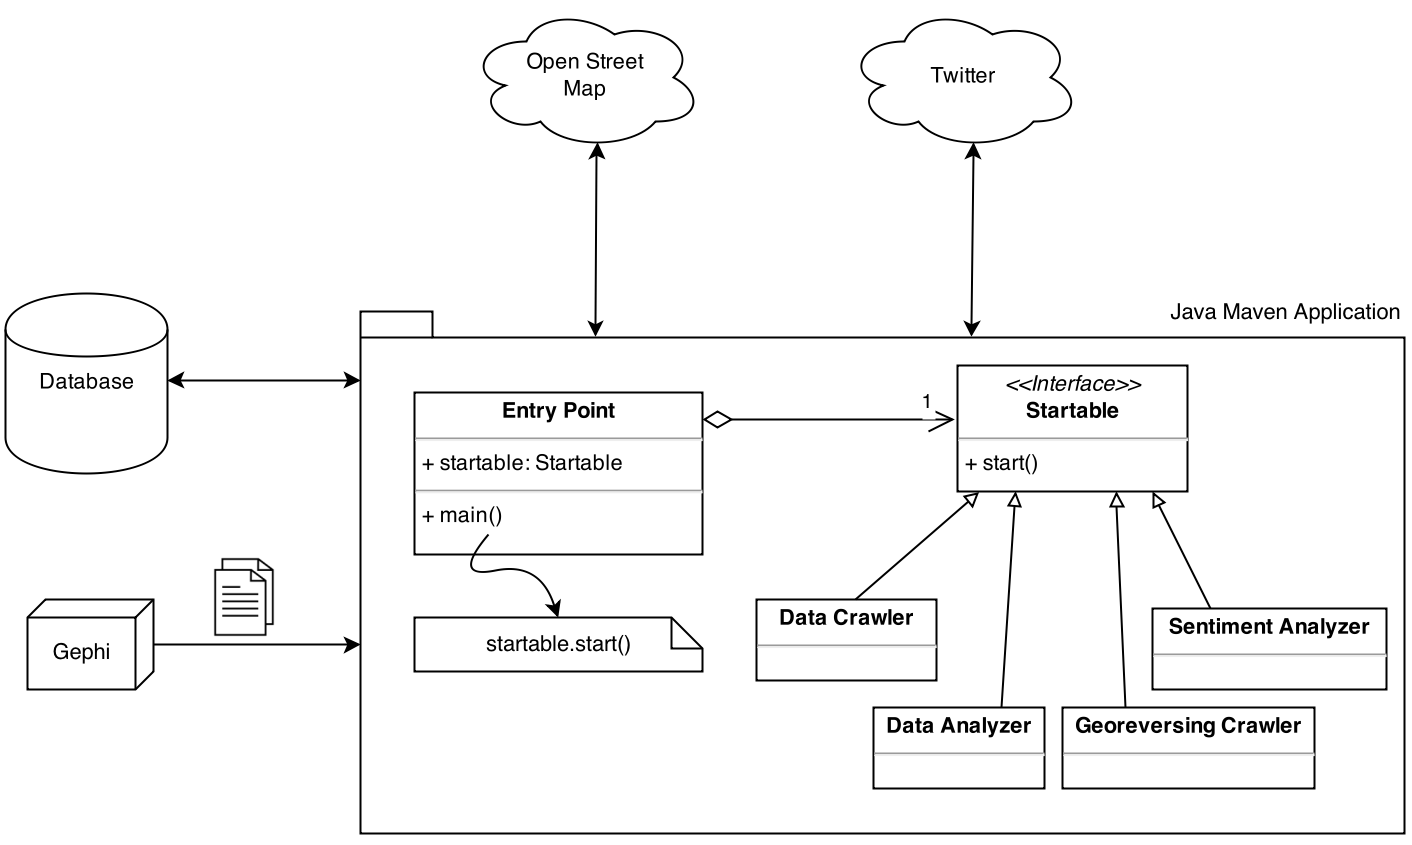
\includegraphics[width=160mm]{img/architektura.png}
\caption{Architektura systemu}
\label{image:architektura-systemu}
\end{figure}
Systemu została zbudowany na pojedynczej aplikacji Javowej,
w której zostały zaimplementowane wszystkie potrzebne operacje.
Aplikacja ta komunikuje się z pojedynczą bazą danych, w której zawarte
są wszystkie wpisy potrzebne zarówno do zbierania danych jak i te, które są
wynikiem analiz. Dodatkowo odpowiada ona za komunikację z usługami w chmurze --
czyli zbieraniem danych z Twittera i \textit{georeversingiem} lokacji z Open
Street Map. Wszystkie analizy zebranych danych również zostały przeprowadzone
przy użyciu aplikacji Javowej.

Oprócz aplikacji Javowej wykorzystano także program Gephi, które wyniki zapisano
do plików, a następnie przy użyciu wyżej wymienionej aplikacji przeparsowano i
umieszczono w bazie danych.

Wewnątrz aplikacji zaimplementowano między innymi moduł do zbierania danych z
Twittera (na podstawie podanych słów kluczowych), moduł związany z
przeprowadzeniem całego procesu analizy sentymentu -- od budowy słownika, do
zanalizowania pojedynczych wpisów, moduł związany z analizą zebranych danych,
a także kod odpowiedzialny za operacje związane z geolokacją.

\section{Zastosowane technologie}
\label{section:zastosowanetechnologie}
% java, postgres, sql, git
Jak już zostało wspomniane wyżej, główną technologią użytą podczas prac był
język Java. Oprócz niego wymienić należy także:
\begin{itemize}
  \item baza danych -- PostgreSQL,
  \item budowanie aplikacji -- Apache Maven,
  \item system kontroli wersji -- Git z repozytorium na GitHub (www.github.com).
\end{itemize}
\section{Wykorzystane biblioteki i narzędzia}
\label{section:bibliotekiinarzedzia}
% Twitter API, CartoDB, OSMap, GMap, GCharts, CartoDB, Gephi
Najważniejsze biblioteki, z których skorzystałem to:
\begin{itemize}
  \item Twitter4J -- biblioteka Javowa ułatwiająca korzystanie z Twitter API,
  użyta do zbierania \mbox{danych z Twittera,}
  \item Hibernate -- framework ORM\footnote{Object Relational Mapping --
  mapowanie obiektowo relacyjne} do komunikacji z bazą danych,
  \item Google Guice, JBoss Weld -- biblioteki pozwalające zastosować
  wstrzykiwanie zależności w aplikacji Javowej,
  \item Google Guava, Apache Commons, Apache Log4J, Joda Time -- biblioteki
  usprawniające programowanie w Javie,
  \item JUnit -- framework do pisania i uruchamiana testów automatycznych.
\end{itemize}